\documentclass[border=10pt]{standalone}

\usepackage{tikz}
\usepackage{tikzsymbols}
\usetikzlibrary{calc,patterns,shapes.geometric}

\def\centerarc[#1](#2)(#3:#4:#5){\draw[#1] ($(#2)+({#5*cos(#3)},{#5*sin(#3)})$) arc (#3:#4:#5);}

\begin{document}
	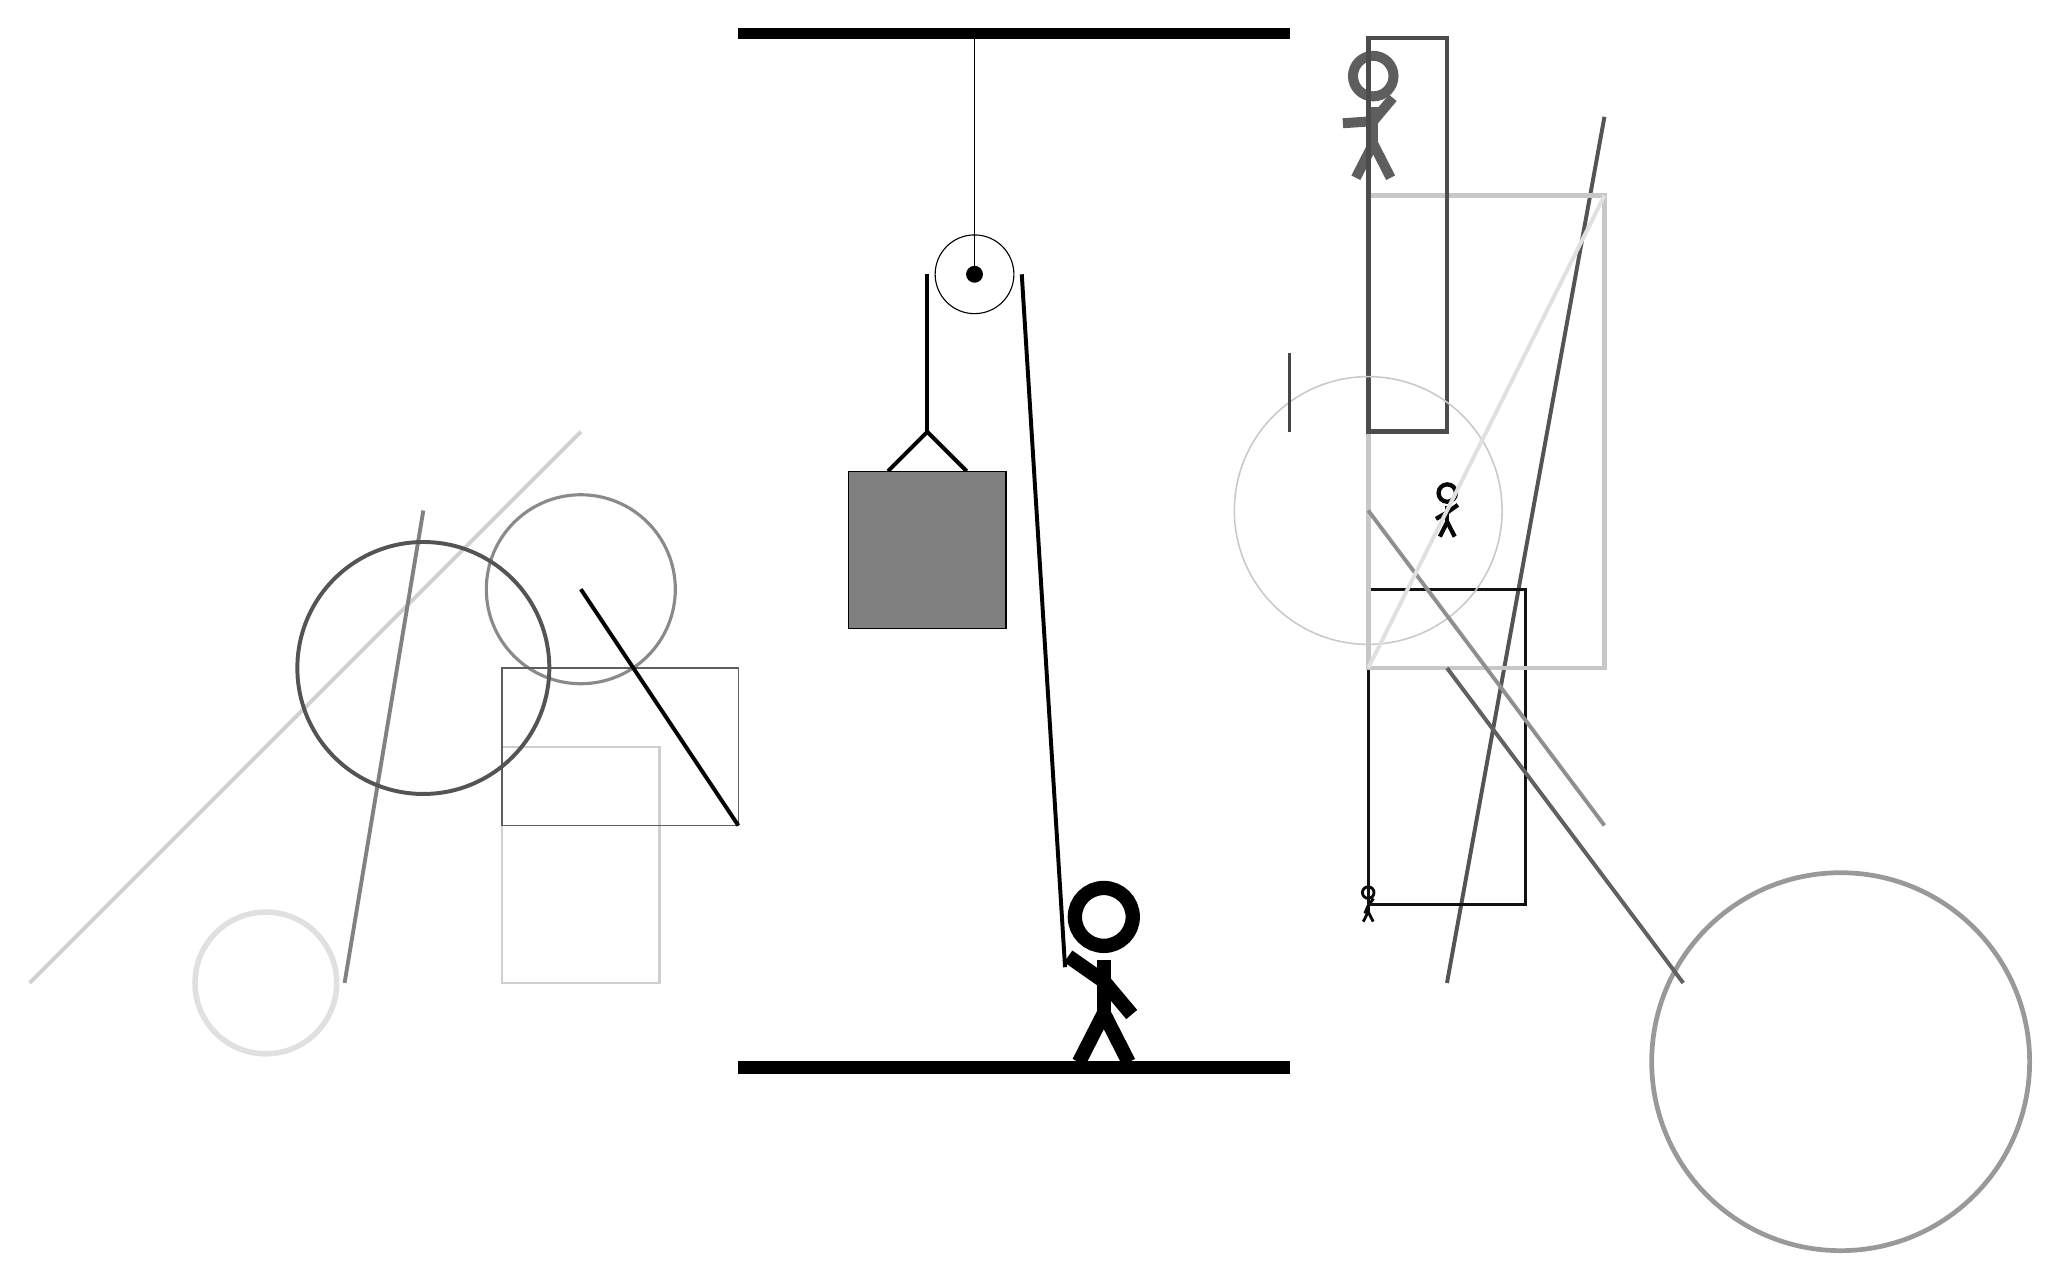
\begin{tikzpicture}
		%%%%% START %%%%%
		
		\draw[fill=black] (-2, 10) rectangle (5, 10.125);
		
		\draw (1, 7) circle (0.5);
		\draw[fill=black] (1, 7) circle (0.1);
		\draw (1, 10) -- (1, 7);
		
		\draw[line width=0.5mm] (-0.1, 4.5) -- (0.4, 5.0) -- (0.9, 4.5);
		\draw[fill=black!50] (-0.6, 4.5) rectangle (1.4, 2.5);
		
		\draw[line width=0.5mm] (0.4, 7) -- (0.4, 5.0);
		\centerarc[line width=0.5mm](1, 7)(0:180:0.6);
		\draw[line width=0.5mm](1.6, 7) -- (2.15, -1.8);
		
		\draw [line width=0.7mm, color=black!12](-8, -2) circle (0.9);
		
		\draw[line width=0.3mm, color=black!19] (-3, -2) rectangle (-5, 1);
		\draw[line width=0.5mm, color=black!14](6, 6) -- (6, 7);
		\node[line width=0.2mm, color=black!63] at (6, 9) {\Strichmaxerl[7][4][50]};
		\draw[line width=0.5mm, color=black!67](9, 9) -- (7, -2);
		
		\node[line width=0.2mm, color=black!97] at (7, 4) {\Strichmaxerl[3][30][35]};
		\draw [line width=0.4mm, color=black!46](-4, 3) circle (1.2);
		\draw[line width=0.2mm, color=black!63] (-2, 0) rectangle (-5, 2);
		\node[line width=0.6mm, color=black!96] at (6, -1) {\Strichmaxerl[2][67][52]};
		\draw[line width=0.4mm, color=black!93] (6, -1) rectangle (8, 3);
		
		\draw[line width=0.5mm, color=black!18](-4, 5) -- (-11, -2);
		
		\draw[line width=0.6mm, color=black!22] (6, 2) rectangle (9, 8);
		\draw[line width=0.6mm, color=black!70] (7, 10) rectangle (6, 5);
		
		\draw [line width=0.2mm, color=black!21](6, 4) circle (1.7);
		\draw[line width=0.5mm, color=black!44](9, 0) -- (6, 4);
		\draw[line width=0.5mm, color=black!98](-2, 0) -- (-4, 3);
		
		\draw[line width=0.5mm, color=black!73](5, 5) -- (5, 6);
		
		\draw[line width=0.5mm, color=black!49](-6, 4) -- (-7, -2);
		\draw [line width=0.6mm, color=black!40](12, -3) circle (2.4);
		\draw[line width=0.5mm, color=black!62](7, 2) -- (10, -2);
		\draw [line width=0.5mm, color=black!67](-6, 2) circle (1.6);
		\draw[line width=0.5mm, color=black!12](9, 8) -- (6, 2);
		
		\node at (2.6, -1.9) {\Strichmaxerl[10][-35][-50]};
		
		\draw[fill=black] (-2, -3) rectangle (5, -3.15);
		
		%%%%% END %%%%%
	\end{tikzpicture}
\end{document}